\documentclass[11pt]{exam}

\usepackage{amsmath, amssymb, multicol}
\usepackage{graphicx}
\usepackage{textcomp}
\usepackage{chessboard}
\usepackage{tikz}

\def\d{\displaystyle}
\def\b{\mathbf}
\def\R{\mathbf{R}}
\def\Z{\mathbf{Z}}
\def\st{~:~}
\def\bar{\overline}
\def\inv{^{-1}}


\newcommand{\vtx}[2]{node[fill,circle,inner sep=0pt, minimum size=4pt,label=#1:#2]{}}
\newcommand{\va}[1]{\vtx{above}{#1}}
\newcommand{\vb}[1]{\vtx{below}{#1}}
\newcommand{\vr}[1]{\vtx{right}{#1}}
\newcommand{\vl}[1]{\vtx{left}{#1}}
\renewcommand{\v}{\vtx{above}{}}


%\pointname{pts}
\pointsinmargin
\marginpointname{pts}
\addpoints
\pagestyle{head}
%\printanswers

\firstpageheader{Math 228}{\bf Counting Matchings}{Monday, April 27}


\begin{document}

%space for name
%\noindent {\large\bf Name:} \underline{\hspace{2.5in}}
%\vskip 1em

\noindent The two richest families in Westeros have decided to enter into an alliance by marriage.  The first family has 10 sons, the second has 10 girls.  The ages of the kids in the two families match up.   To avoid impropriety, the families insist that each child must marry someone either their own age, or someone one position younger or older.  In fact, the graph representing agreeable marriages looks like this:

\begin{center}
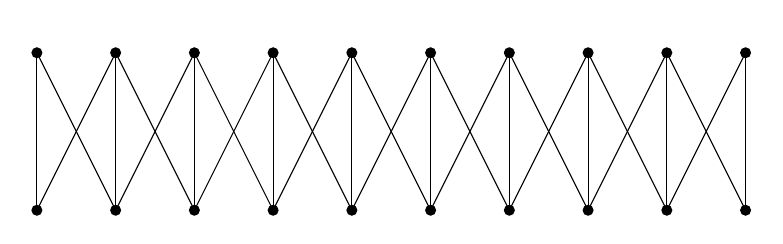
\begin{tikzpicture}
\foreach \x in {0,...,9} {
 \coordinate (a\x) at (\x,0);
 \coordinate (b\x) at (\x,2);
 \draw (a\x) \v -- (b\x) \v;
 }
\draw (a0) -- (b1) -- (a2) -- (b3) -- (a4) -- (b5) -- (a6) -- (b7) -- (a8) -- (b9);
\draw (b0) -- (a1) -- (b2) -- (a3) -- (b4) -- (a5) -- (b6) -- (a7) -- (b8) -- (a9);

\end{tikzpicture}
\end{center}  

The question: how many different acceptable marriage arrangements which marry off all 20 children are possible?

\begin{questions}
\question How many marriage arrangements are possible if we insist that there are exactly 6 boys marry girls not their own age?  
\vfill

\question Could you generalize the previous answer to arrive at the total number of marriage arrangements?

\vfill

\question How do you know you are correct?  Try counting in a different way.  Look at smaller family sizes and get a sequence.

\vfill

\question Can you give a recurrence relation that fits the problem?  

\vfill


\end{questions}

\end{document}


